\switchcolumn[1]
\codeblock{basics/mc_fishers}

\begin{figure}[!h]
  \centering
  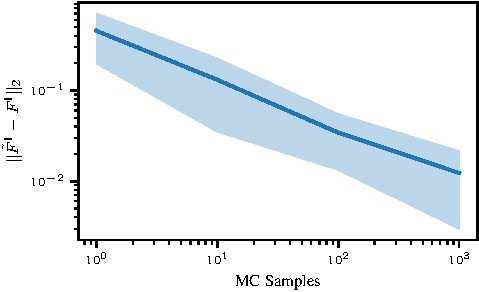
\includegraphics[width=\linewidth]{../kfs/plots/synthetic_rvec_diff_spec_norm.pdf}
  \caption{ \textbf{Convergence of the Monte Carlo-approximated type-I Fisher to the type-I Fisher.}
    We visualize spectral norm of their residual as a function of MC samples.
    The Fishers were evaluated on synthetic data ($N=100$) using an MLP with three fully-connected layers and ReLU activations (5-4-4-3) and square loss.
    In this setting, the exact type-I Fisher equals the GGN, and we used GGNVPs (\Cref{def:ggnvp}) to compute it.
    Plot produced with \repofile{plots/synthetic_fisher}.
  }\label{fig:mc-fisher-converges-to-fisher}
\end{figure}

\codeblock{basics/mc_fisher_product}
\switchcolumn[0]

\paragraph{Recap: Probabilistic interpretation.}
In \Cref{subsec:probabilistic-interpretation} we demonstrated that a neural net often models a likelihood for the labels given the inputs using parameters.
This probabilistic perspective provides a new way to compare two models $f_1 \coloneq f(\bullet, \vtheta_1), f_2 \coloneq f(\bullet, \vtheta_{2})$ where $\vtheta_2 = \vtheta_1 + \Delta \vtheta$: Instead of assessing their dissimilarity by their parameters' dissimilarity, \eg using the Euclidean distance measure $d^2(f_1, f_2) = \left\lVert \vtheta_2 - \vtheta_1 \right\rVert_2^2 = \left\lVert \Delta \vtheta \right\rVert_2^2$, we can instead use the KL divergence of the represented probability densities, $d^2(f_1, f_2) = \mathrm{KL}(p(\rvx, \rvy \mid \vtheta_1) \mid\mid p(\rvx, \rvy \mid \vtheta_2))$.

\paragraph{The Fisher as metric of the KL divergence.}
Using $p(\rvx, \rvy \mid \vtheta) = p(\rvy \mid \rvx, \vtheta)p_{\text{data}}(\rvx)$, we have
\begin{align*}
  & \mathrm{KL}(p(\rvx, \rvy \mid \vtheta_1) \mid\mid p(\rvx, \rvy \mid \vtheta_2))                               \\
  = & \E_{p_{\text{data}}(\rvx)} [\mathrm{KL}(p(\rvy \mid \rvx, \vtheta_1) \mid\mid p(\rvy \mid \rvx, \vtheta_2))].
\end{align*}
While the KL divergence is not a valid distance measure for general pairs $(\vtheta_1, \vtheta_2)$ (\eg it is not symmetric \wrt its arguments), it can be locally approximated by a quadratic Taylor series for small $\Delta \vtheta$.
The curvature matrix in that Taylor series is the Fisher,
\begin{align*}
  \mathrm{KL}(p(\rvx, \rvy \mid \vtheta) \mid\mid p(\rvx, \rvy \mid \vtheta + \Delta \vtheta))
  \\
  = \frac{1}{2} {\Delta \vtheta}^{\top} \mF(\vtheta) \Delta \vtheta + \gO( \Vert\Delta \vtheta\Vert^3)\,,
\end{align*}
with the Fisher information matrix
\begin{align*}
  \mF(\vtheta) &\coloneqq \E_{p(\rvx, \rvy \mid \vtheta)} [-\hess_{\vtheta} \log p(\rvx, \rvy \mid \vtheta)]\,.
                 \shortintertext{Let's rewrite this expression in terms of the likelihood $p(\rvy \mid \vx, \vtheta)$, and its reparameterized likelihood $r(\rvy \mid f(\rvx, \vtheta))$ with the neural net prediction,}
  &= \E_{p_{\text{data}}(\rvx)}\E_{p(\rvy \mid \rvx, \vtheta)} [-\hess_{\vtheta} \log p(\rvy \mid \rvx, \vtheta)]
  \\
               &=
                 \E_{p_{\text{data}}(\rvx)}\E_{r(\rvy \mid f(\rvx, \vtheta))} [
  \\
               &\qquad\qquad\qquad-\hess_{\vtheta} \log r(\rvy \mid f(\rvx, \vtheta))]\,.
\end{align*}
The expectation over the data-generating distribution's marginal $p_{\text{data}}(\rvx)$ is intractable.
Therefore, we will replace it with the empirical distribution over our data set in the following.
Following \citet{soen2024tradeoffs}, we present two forms of the Fisher: While the \emph{type-II Fisher} allows to elegantly connect the Fisher and the GGN and highlights its connection to the Hessian (a curvature matrix), the \emph{type-I Fisher} highlights that the Fisher is a gradient covariance matrix, and can therefore be computed with first-order derivatives.

\paragraph{Type-II Fisher.}
Let's replace the true marginal distribution over the inputs with its empirical distribution $p_{\sD}(\rvx) = \frac{1}{N}\sum_n \delta(\rvx - \vx_n)$.
This yields the type-II Fisher information matrix (because it is defined via second-order derivatives),
\begin{align*}
  \mF^{\text{II}}(\vtheta)
  & =
    \E_{p_{\sD}(\rvx)}\E_{r(\rvy \mid f(\rvx, \vtheta))} [
  \\
  &\qquad\qquad\qquad
    -\hess_{\vtheta} \log r(\rvy \mid f(\rvx, \vtheta))]
  \\
  & =
    \frac{1}{N} \sum_n
    \E_{r(\rvy \mid \vf_n)} [-\hess_{\vtheta} \log r(\rvy \mid \vf_n)]
    \shortintertext{(remember $\vf_n \coloneq f(\rvx = \vx_n, \vtheta)$).
    We can apply the chain rule to the log-likelihood's Hessian (remember the 1d example from \Cref{sec:partial_linearization}) and use that $\E_{r(\rvy \mid f(\rvx, \vtheta))}[\nabla_{f(\rvx, \vtheta)} \log r(\rvy \mid f(\rvx, \vtheta))] = \vzero$ to simplify the type-II Fisher into}
  &= \frac{1}{N} \sum_n \E_{r(\rvy \mid \vf_n)} [
    \begin{aligned}[t]
      & {\jac_{\vtheta} \vf_n}^{\top}                          \\
      & \left( -\hess_{\vf_n} \log r(\rvy \mid \vf_n)  \right) \\
      & \jac_{\vtheta} \vf_n ]\,
    \end{aligned}
    \shortintertext{and, as Jacobians do not depend on $\rvy$,}
  & = \frac{1}{N} \sum_n
    \begin{aligned}[t]
      & {\jac_{\vtheta} \vf_n}^{\top} \\
      & \left(
        \E_{r(\rvy \mid \vf_n)} [
        -\hess_{\vf_n} \log r(\rvy \mid \vf_n)
        ]
        \right)                          \\
      & \jac_{\vtheta} \vf_n \,.
    \end{aligned}
\end{align*}
This form resembles a lot the GGN.
In fact, for square loss and softmax cross-entropy loss ($c = - \log$), we derived that the loss Hessian we average in the type-II Fisher does not depend on the labels modelled by the distribution (see \Cref{ex:hessian-crossentropyloss,ex:square_loss_hessian}).
This means we can drop the expectation for such losses.
We just showed that the (type-II) \emph{Fisher equals the GGN for regression with square loss and classification with softmax cross-entropy loss} (more details in \Cref{subsec:connection-ggn-fisher}).

\paragraph{Type-I Fisher.} There is another way to rewrite the Fisher in terms of first-order derivatives of the log-likelihood.
We will call this the type-I Fisher information matrix.
To derive it, we use the property that the negative log-likelihood's Hessian equals its gradient covariance in expectation,
\begin{align*}
  & \E_{p(\rvx, \rvy \mid \vtheta)}
    \left[
    -\hess_{\vtheta} \log p(\rvx, \rvy \mid \vtheta)
    \right]
  \\
  = & \E_{p(\rvx, \rvy \mid \vtheta)} [
      \begin{aligned}[t]
        & (-\nabla_{\vtheta} \log p(\rvx, \rvy \mid \vtheta)) \\
        & (-\nabla_{\vtheta} \log p(\rvx, \rvy\mid  \vtheta))^{\top}]
      \end{aligned}
\end{align*}
Hence, we can write the Fisher as
\begin{align*}
  &\mF(\vtheta)
  \\
  & = \E_{p(\rvx, \rvy \mid \vtheta)} [
    \begin{aligned}[t]
      & (-\nabla_{\vtheta} \log p(\rvx, \rvy \mid \vtheta))        \\
      & (-\nabla_{\vtheta} \log p(\rvx, \rvy \mid \vtheta))^{\top}]
    \end{aligned}
    \shortintertext{(factorize $p(\rvx, \rvy \mid \vtheta) = p_{\text{data}}(\rvx) p(\rvy \mid \rvx, \vtheta)$)}
  & = \E_{p_{\text{data}}(\rvx)}\E_{p(\rvy \mid \rvx, \vtheta))} [
    \begin{aligned}[t]
      & (-\nabla_{\vtheta} \log p(\rvy \mid \rvx, \vtheta))        \\
      & (-\nabla_{\vtheta} \log p(\rvy \mid \rvx, \vtheta))^{\top}]
    \end{aligned}
    \shortintertext{(reparameterize $p(\rvy \mid \rvx, \vtheta) = r(\rvy \mid f(\rvx, \vtheta))$)}
  & = \E_{p_{\text{data}}(\rvx)}\E_{r(\rvy \mid f(\rvx, \vtheta))} [
  \\
  &\qquad \qquad\qquad
    (-\nabla_{\vtheta} \log r(\rvy \mid f(\rvx, \vtheta)))
  \\
  &\qquad \qquad\qquad
    (-\nabla_{\vtheta} \log r(\rvy \mid f(\rvx, \vtheta)))^{\top}]
\end{align*}
Let's apply the chain rule for the gradient, substitute the empirical distribution for $p_{\text{data}}(\rvx)$ and simplify.
This gives the type-I Fisher
\begin{align*}
  & \mF^{\text{I}}(\vtheta)
  \\
  & =
    \frac{1}{N} \sum_n
    \E_{r(\rvy \mid \vf_n)}
    [\begin{aligned}[t]
      & (-\nabla_{\vtheta} \log r(\rvy \mid \vf_n)) \\
      & (-\nabla_{\vtheta} \log r(\rvy \mid \vf_n))^{\top}]
    \end{aligned}
  \\
  & =
    \frac{1}{N} \sum_n
    \E_{r(\rvy \mid \vf_n)}
    [\begin{aligned}[t]
      & (\jac_{\vtheta}\vf_n)^{\top} \\
      & (-\nabla_{\vf_n} \log r(\rvy \mid \vf_n)) \\
      & (-\nabla_{\vf_n} \log r(\rvy \mid \vf_n))^{\top} \\
      & \jac_{\vtheta}\vf_n]
    \end{aligned}
  \\
  \shortintertext{and, as the Jacobians do not depend on $\rvy$,}
  & =
    \frac{1}{N} \sum_n
    \begin{aligned}[t]
      & (\jac_{\vtheta}\vf_n)^{\top} \\
      & \E_{r(\rvy \mid \vf_n)}
        [(-\nabla_{\vf_n} \log r(\rvy \mid \vf_n)) \\
      & \phantom{\E_{r(\rvy \mid \vf_n)}[}(-\nabla_{\vf_n} \log r(\rvy \mid \vf_n))^{\top}] \\
      & \jac_{\vtheta}\vf_n \,.
    \end{aligned}
\end{align*}
This form highlights that the Fisher can be computed with first-order derivatives, specifically vector-Jacobian products.

\paragraph{Monte Carlo-approximated type-I Fisher.} For computations with the type-I Fisher, we need to replace the expectation over $r(\rvy \mid \vf_n)$ with an estimator, \eg Monte Carlo approximation with $M$ sampled labels $\smash{\tilde{\vy}_{n,1}, \dots, \tilde{\vy}_{n, M} \stackrel{\text{i.i.d}}{\sim} r(\rvy \mid \vf_n)}$ for the prediction of datum $n$.
Thankfully, we already developed the functionality to sample such labels in \Cref{subsec:probabilistic-interpretation} (specifically, \Cref{basics/label_sampling}).

\begin{definition}[Monte Carlo-approximated type-I Fisher (\Cref{basics/mc_fishers})]\label{def:mc_fisher}%
  The Monte Carlo-approximated type-I Fisher of the likelihood $\log r(\rvy \mid f(\vx_n, \vtheta))$,
  $\tilde{\mF}^{\text{I}}(\vtheta) \in \sR^{D \times D}$ is
  \begin{align*}
    & \tilde{\mF}^{\text{I}}(\vtheta) \\
    & = \frac{1}{NM} \sum_{n,m}
      \begin{aligned}[t]
        & (-\nabla_{\vtheta} \log r(\rvy = \tilde{\vy}_{n,m} \mid \vf_n))        \\
        & (-\nabla_{\vtheta} \log r(\rvy = \tilde{\vy}_{n,m} \mid \vf_n))^{\top} \\
      \end{aligned} \\
    & = \frac{1}{NM} \sum_{n,m}
      \begin{aligned}[t]
        & \left(\jac_{\vtheta}\vf_n\right)^{\top}                              \\
        & (-\nabla_{\vf_n} \log r(\rvy = \tilde{\vy}_{n,m} \mid \vf_n))        \\
        & (-\nabla_{\vf_n} \log r(\rvy = \tilde{\vy}_{n,m} \mid \vf_n))^{\top} \\
        & \jac_{\vtheta}\vf_n.
      \end{aligned}
  \end{align*}
\end{definition}
As we increase the number of Monte Carlo (MC) samples, the the MC-approximated type-I Fisher converges to the Fisher, as illustrated in \Cref{fig:mc-fisher-converges-to-fisher}.

\paragraph{Would-be gradients \& self-outer product form.}
To compute with the type-I Fisher, we need to evaluate gradient of the loss using sampled labels, rather than the labels from the data set (see \Cref{basics/mc_fisher_product}, which implements multiplication with the MC Fisher).
As coined by \citet{papyan2020traces}, we call these gradients `would-be' gradients, because they depend on hypothetical labels.

Let's denote the $m$-th negative would-be gradient for sample $n$ by $\tilde{\vg}_{n,m} \coloneq -\nabla_{\vf_n} \log r(\rvy = \tilde{\vy}_{n,m} \mid \vf_n)$
We can then form the matrix
\begin{align*}
  \tilde{\mS}_n
  \coloneq
  \frac{1}{\sqrt{M}}
  \begin{pmatrix}
    \tilde{\vg}_{n,1} & \cdots & \tilde{\vg}_{n,M}
  \end{pmatrix}
  \in \sR^{\dim(\gF) \times M}
\end{align*}
for each $n$, and express the MC Fisher as
\begin{align*}
  \tilde{\mF}^{\text{I}}(\vtheta)
  & =
    \frac{1}{N} \sum_{n,m}
    (\jac_{\vtheta}\vf_n)^{\top}
    \tilde{\mS}_n
    \tilde{\mS}_n^{\top}
    (\jac_{\vtheta}\vf_n)
  \\
  & =
    \frac{1}{N} \sum_n
    \tilde{\mV}_n
    \tilde{\mV}_n^{\top}
\end{align*}
where $\tilde{\mV}_n = (\jac_{\vtheta}\vf_n)^{\top} \tilde{\mS}_n \in \sR^{D \times M}$.

Did you notice what we just did here?
By stacking the negative would-be gradients into columns of a matrix, we were able to express the Fisher as the self-outer product of a matrix $\tilde{\mV}_n$.
This notation looks very similar to the GGN's self-outer product notation.
In fact, we can think of $\tilde{\mV}_n \in \sR^{D \times M}$ as a \emph{randomization} of $\mV_n \in \sR^{D \times C}$ which can be much smaller (depending on $M$) and therefore cheaper to compute in exchange for inaccuracy.
The different self-outer product forms of curvature matrices will give rise to multiple flavours of KFAC in \Cref{sec:kfac-overview}.

\paragraph{Reduction factor of the Fisher vs.\,empirical risk.}
In the above derivation we arrived at an expression of the Fisher which uses a reduction factor $R = \nicefrac{1}{N}$.
We will handle this factor flexibly in practise by using the reduction factor of our empirical risk.

\paragraph{(Optional) efficient would-be gradient computation.}
One way to compute would-be gradients is to repeatedly sample a label, compute its loss, then use automatic differentiation to obtain the gradient.
This incurs \texttt{for} loops, which may be sub-optimal for performance.
In this tutorial, we follow the less efficient \texttt{for} loop approach as it is less complex.
To improve efficiency, we could draw all labels in parallel, and compute their gradients manually instead of using autodiff, which is cheaper as demonstrated by \Cref{ex:square-loss-gradient,ex:cross-entropy-loss-gradient}.
They provide the gradients of square loss and softmax cross-entropy loss, which are straightforward to evaluate manually.
However, we will not apply this optimization in our tutorial.

\switchcolumn[1]
\begin{example}[Gradients of square loss]\label{ex:square-loss-gradient}
  Consider the square loss from \Cref{ex:square_loss} and its probabilistic interpretation from \Cref{ex:square_loss_probabilistic}
  For some label $\vy$, the gradient is given by
  \begin{align*}
    \nabla_{\vf} c(\vf, \vy)
    & =
      - \nabla_{\vf} \log r(\rvy =\vy \mid \vf)
    \\
    & =
      \vf - \vy\,.
  \end{align*}
\end{example}

\begin{example}[Gradients of softmax cross-entropy loss]\label{ex:cross-entropy-loss-gradient}
  Consider the softmax cross-entropy loss from \Cref{ex:cross_entropy_loss} and its probabilistic interpretation from \Cref{ex:cross_entropy_loss_probabilistic}. For some label $y$, the gradient is given by
  \begin{align*}
    \nabla_{\vf} c(\vf, y)
    & =
      - \nabla_{\vf} \log r(\ry = y \mid \vf)
    \\
    & =
      \vsigma(\vf) - \mathrm{onehot}(y)\,.
  \end{align*}
\end{example}
\switchcolumn[0]
%%% Local Variables:
%%% mode: latex
%%% TeX-master: "../main"
%%% End:
